\documentclass[11pt,a4paper]{article}

% ======================
% Packages
% ======================

\usepackage[utf8]{inputenc}
\usepackage[T1]{fontenc}
\usepackage{lmodern}
\usepackage{amsmath}
\usepackage{amsfonts}
\usepackage{amssymb}
\usepackage{graphicx}
\usepackage{booktabs}
\usepackage{geometry}
\usepackage{setspace}
\usepackage{cite}
\usepackage{float}

\geometry{margin=2.5cm}
\setstretch{1.15}

% ======================
% Document
% ======================

\begin{document}

\title{Gap-Based Structural Equation Model for University Sustainability Assessment}

\author{Author Name}

\date{}

\maketitle

% =====================================================
\section{Gap-Based Structural Equation Model for University Sustainability Assessment}
% =====================================================



\subsection{Conceptual Foundation of the Gap-Based Sustainability Model}

Based on the qualitative analysis conducted with the university’s core stakeholders, sustainability emerges as a multidimensional latent construct encompassing economic, social, and environmental dimensions. The findings reveal that sustainability cannot be adequately characterized solely by the existence of technical initiatives or institutional policies, but must also incorporate how these initiatives are perceived and evaluated by stakeholders. In this perspective, sustainability is not only an operational outcome but also a perceptual and relational construct shaped by stakeholder experience and interpretation.

The qualitative results highlighted a systematic divergence between stakeholder perceptions of existing sustainability initiatives and their expectations regarding institutional sustainability performance. While several operational actions were identified across economic, social, and environmental domains, stakeholders frequently emphasized limitations related to their visibility, institutionalization, and strategic alignment. This divergence reflects a structural misalignment between institutional sustainability efforts and stakeholder priorities, which cannot be captured through traditional performance indicators alone.

To address this limitation, the present study introduces the Expectation--Perception Gap as a central conceptual construct for sustainability assessment. This gap represents the difference between stakeholder expectations and their perception of the implemented sustainability initiatives. Conceptually, it captures the degree of alignment between institutional sustainability performance and stakeholder priorities. A smaller gap indicates stronger alignment and greater perceived sustainability effectiveness, whereas a larger gap reflects structural misalignment and reduced sustainability coherence.

Within this framework, sustainability is modeled as a hierarchical latent construct structured around three core dimensions: economic sustainability, social sustainability, and environmental sustainability. Each dimension is influenced by stakeholder perception and stakeholder expectation, and their interaction determines the level of alignment between institutional performance and stakeholder priorities.

Building upon this gap-centered perspective, the University Sustainability Index (USI) is introduced as an integrative latent construct representing the overall level of institutional sustainability. Rather than relying solely on operational performance indicators, the USI reflects the degree of alignment between institutional sustainability initiatives and stakeholder expectations. This formulation provides a stakeholder-centered and behaviorally grounded representation of sustainability, enabling a more comprehensive and realistic assessment of institutional sustainability performance.


\subsection{Definition of Latent Variables and Constructs}

In order to formalize the proposed sustainability framework, university sustainability is modeled using latent variables representing stakeholder perception, stakeholder expectation, sustainability alignment, and overall institutional sustainability performance. These constructs are not directly observable but are inferred through observed indicators derived from stakeholder responses.

The model distinguishes between exogenous latent variables, which represent perceived and expected sustainability, and endogenous latent variables, which represent the sustainability gaps and the overall University Sustainability Index.

The vector of exogenous latent variables is defined as:

\begin{equation}
\xi =
\begin{bmatrix}
P_e \\
P_s \\
P_{env} \\
E_e \\
E_s \\
E_{env}
\end{bmatrix}
\end{equation}

where:

\begin{itemize}
\item Perceived Economic Sustainability ($P_e$), reflecting stakeholder evaluation of existing economic sustainability initiatives, such as digitalization, resource optimization, and institutional efficiency;
\item Perceived Social Sustainability ($P_s$), reflecting stakeholder perception of inclusion, well-being, social engagement, and institutional support mechanisms;
\item Perceived Environmental Sustainability ($P_{env}$), reflecting stakeholder perception of environmental initiatives, including waste management, resource conservation, and ecological awareness;
\item Expected Economic Sustainability ($E_e$), reflecting stakeholder expectations regarding economic sustainability performance and institutional commitment;
\item Expected Social Sustainability ($E_s$), reflecting stakeholder expectations concerning inclusion, psychological support, and social responsibility;
\item Expected Environmental Sustainability ($E_{env}$), reflecting stakeholder expectations regarding environmental protection, resource management, and ecological institutionalization.
\end{itemize}

These exogenous latent variables capture stakeholder-based evaluations of institutional sustainability performance from both perceptual and normative perspectives.

The vector of endogenous latent variables is defined as:

\begin{equation}
\eta =
\begin{bmatrix}
G_e \\
G_s \\
G_{env} \\
USI
\end{bmatrix}
\end{equation}

where:

\begin{itemize}
\item Economic Sustainability Gap ($G_e$), representing the alignment between perceived and expected economic sustainability;
\item Social Sustainability Gap ($G_s$), representing the alignment between perceived and expected social sustainability;
\item Environmental Sustainability Gap ($G_{env}$), representing the alignment between perceived and expected environmental sustainability.
\end{itemize}

The sustainability gap for each dimension represents the degree of alignment between stakeholder expectations and perceived institutional sustainability performance, and is defined as:

\begin{equation}
G_e = E_e - P_e
\end{equation}

\begin{equation}
G_s = E_s - P_s
\end{equation}

\begin{equation}
G_{env} = E_{env} - P_{env}
\end{equation}

These gap variables act as mediating latent constructs that capture the alignment between institutional sustainability initiatives and stakeholder priorities.

The University Sustainability Index is defined as a higher-order latent construct integrating the sustainability gaps across the three dimensions. It can be expressed as a linear combination of the sustainability gaps:

\begin{equation}
USI = \beta_1 G_e + \beta_2 G_s + \beta_3 G_{env} + \zeta
\end{equation}

where:

\begin{itemize}
\item $\beta_1, \beta_2, \beta_3$ represent the contribution weights of economic, social, and environmental sustainability gaps, respectively,
\item $\zeta$ represents the structural disturbance term.
\end{itemize}

This formulation establishes the University Sustainability Index as a stakeholder-centered latent construct reflecting the degree of alignment between institutional sustainability performance and stakeholder expectations.

The vector representation of the latent variables provides the mathematical foundation for specifying both the measurement model and the structural model within the structural equation modeling framework.



\subsection{Measurement Model Specification}

The measurement model defines the relationships between latent variables and their corresponding observed indicators. In the proposed framework, the measurement model specifies how perceived sustainability, expected sustainability, sustainability gaps, and the overall sustainability index are inferred from observed stakeholder responses.

The measurement model consists of two components: the exogenous measurement model and the endogenous measurement model.

\subsubsection{Exogenous Measurement Model}

The exogenous measurement model defines the relationships between observed indicators and the exogenous latent variables representing perceived and expected sustainability. It is expressed in matrix form as:

\begin{equation}
x = \Lambda_x \xi + \delta
\end{equation}

where:

\begin{itemize}
\item $x$ is the vector of observed indicators measuring perceived and expected sustainability,
\item $\Lambda_x$ is the loading matrix relating observed indicators to exogenous latent variables,
\item $\xi$ is the vector of exogenous latent variables defined in Equation (1),
\item $\delta$ is the vector of measurement errors associated with exogenous indicators.
\end{itemize}

The observed indicator vector is defined as:

\begin{equation}
x =
\begin{bmatrix}
x_1 \\
x_2 \\
\vdots \\
x_p
\end{bmatrix}
\end{equation}

where each observed variable represents a stakeholder-based indicator of perceived or expected sustainability across economic, social, and environmental dimensions.

Each observed indicator is assumed to be linearly related to its corresponding latent construct. For example, perceived economic sustainability is measured through observed indicators related to digitalization, resource optimization, and institutional efficiency, while expected sustainability is measured through stakeholder expectations regarding institutional sustainability performance.

\subsubsection{Endogenous Measurement Model}

The endogenous measurement model defines the relationships between observed indicators and endogenous latent variables representing sustainability gaps and the University Sustainability Index. It is expressed as:

\begin{equation}
y = \Lambda_y \eta + \epsilon
\end{equation}

where:

\begin{itemize}
\item $y$ is the vector of observed indicators measuring sustainability gaps and institutional sustainability performance,
\item $\Lambda_y$ is the loading matrix relating observed indicators to endogenous latent variables,
\item $\eta$ is the vector of endogenous latent variables defined in Equation (2),
\item $\epsilon$ is the vector of measurement errors associated with endogenous indicators.
\end{itemize}

The observed indicator vector is defined as:

\begin{equation}
y =
\begin{bmatrix}
y_1 \\
y_2 \\
\vdots \\
y_q
\end{bmatrix}
\end{equation}

These observed indicators reflect stakeholder-perceived alignment between institutional sustainability initiatives and stakeholder expectations, as well as the overall institutional sustainability performance.

\subsubsection{Measurement Model Interpretation}

The loading matrices $\Lambda_x$ and $\Lambda_y$ define the strength of the relationships between observed indicators and their corresponding latent constructs. Higher loading values indicate stronger relationships between observed variables and latent variables, reflecting higher construct validity.

The measurement errors $\delta$ and $\epsilon$ represent measurement uncertainty and unobserved influences affecting the observed indicators.

This measurement model establishes the empirical link between stakeholder responses and latent sustainability constructs, ensuring that perceived sustainability, expected sustainability, sustainability gaps, and the University Sustainability Index are properly represented within the structural equation modeling framework.



\section{Methodology}

\subsection{Research Design}

This study adopts a qualitative stakeholder-centered research design aimed at identifying the key dimensions of university sustainability from the perspective of its core community. The research framework is grounded in stakeholder theory and alignment-based sustainability assessment, focusing on the divergence between perceived and expected sustainability.

The study follows an exploratory-to-structural approach, where qualitative insights are first collected and analyzed, and subsequently formalized into a latent variable framework for sustainability assessment.

\subsection{Stakeholder Selection}

Two primary stakeholder groups were considered:

\begin{itemize}
\item Students
\item Academic staff (teachers)
\end{itemize}

These stakeholders were selected because they directly interact with institutional sustainability initiatives and represent the internal academic community. Their perceptions and expectations provide essential insights into the effectiveness and alignment of sustainability strategies.

\subsection{Data Collection}

Data were collected using structured questionnaires designed to capture both perceived sustainability and expected sustainability across three core dimensions:

\begin{itemize}
\item Economic sustainability
\item Social sustainability
\item Environmental sustainability
\end{itemize}

Each dimension was measured using multiple indicators reflecting operational initiatives, institutional support mechanisms, and sustainability-related practices.

Responses were collected using Likert-type scales to quantify stakeholder evaluations of sustainability performance and expectations.

\subsection{Construction of Sustainability Dimensions}

Based on qualitative analysis of stakeholder responses, sustainability was conceptualized as a multidimensional construct. For each dimension, two latent constructs were defined:

\begin{itemize}
\item Perceived sustainability
\item Expected sustainability
\end{itemize}

The sustainability gap was operationalized as the difference between expected and perceived sustainability for each dimension. This gap represents the degree of alignment between institutional sustainability actions and stakeholder expectations.

\subsection{Model Development Strategy}

The qualitative findings were translated into a latent variable framework using structural equation modeling principles. The measurement structure defines how observed questionnaire indicators relate to latent sustainability constructs, while the index formulation integrates the sustainability gaps into a unified University Sustainability Index.

This methodological approach ensures theoretical consistency, construct validity, and a stakeholder-centered representation of university sustainability.


\subsection{Structural Model Specification}

The structural model defines the causal relationships between the latent variables representing perceived sustainability, expected sustainability, sustainability gaps, and the overall University Sustainability Index. It formalizes how stakeholder perception and stakeholder expectation influence sustainability alignment, and how this alignment determines institutional sustainability performance.

Figure \ref{fig:sem_model} illustrates the proposed structural equation model.

\begin{figure}[H]
\centering
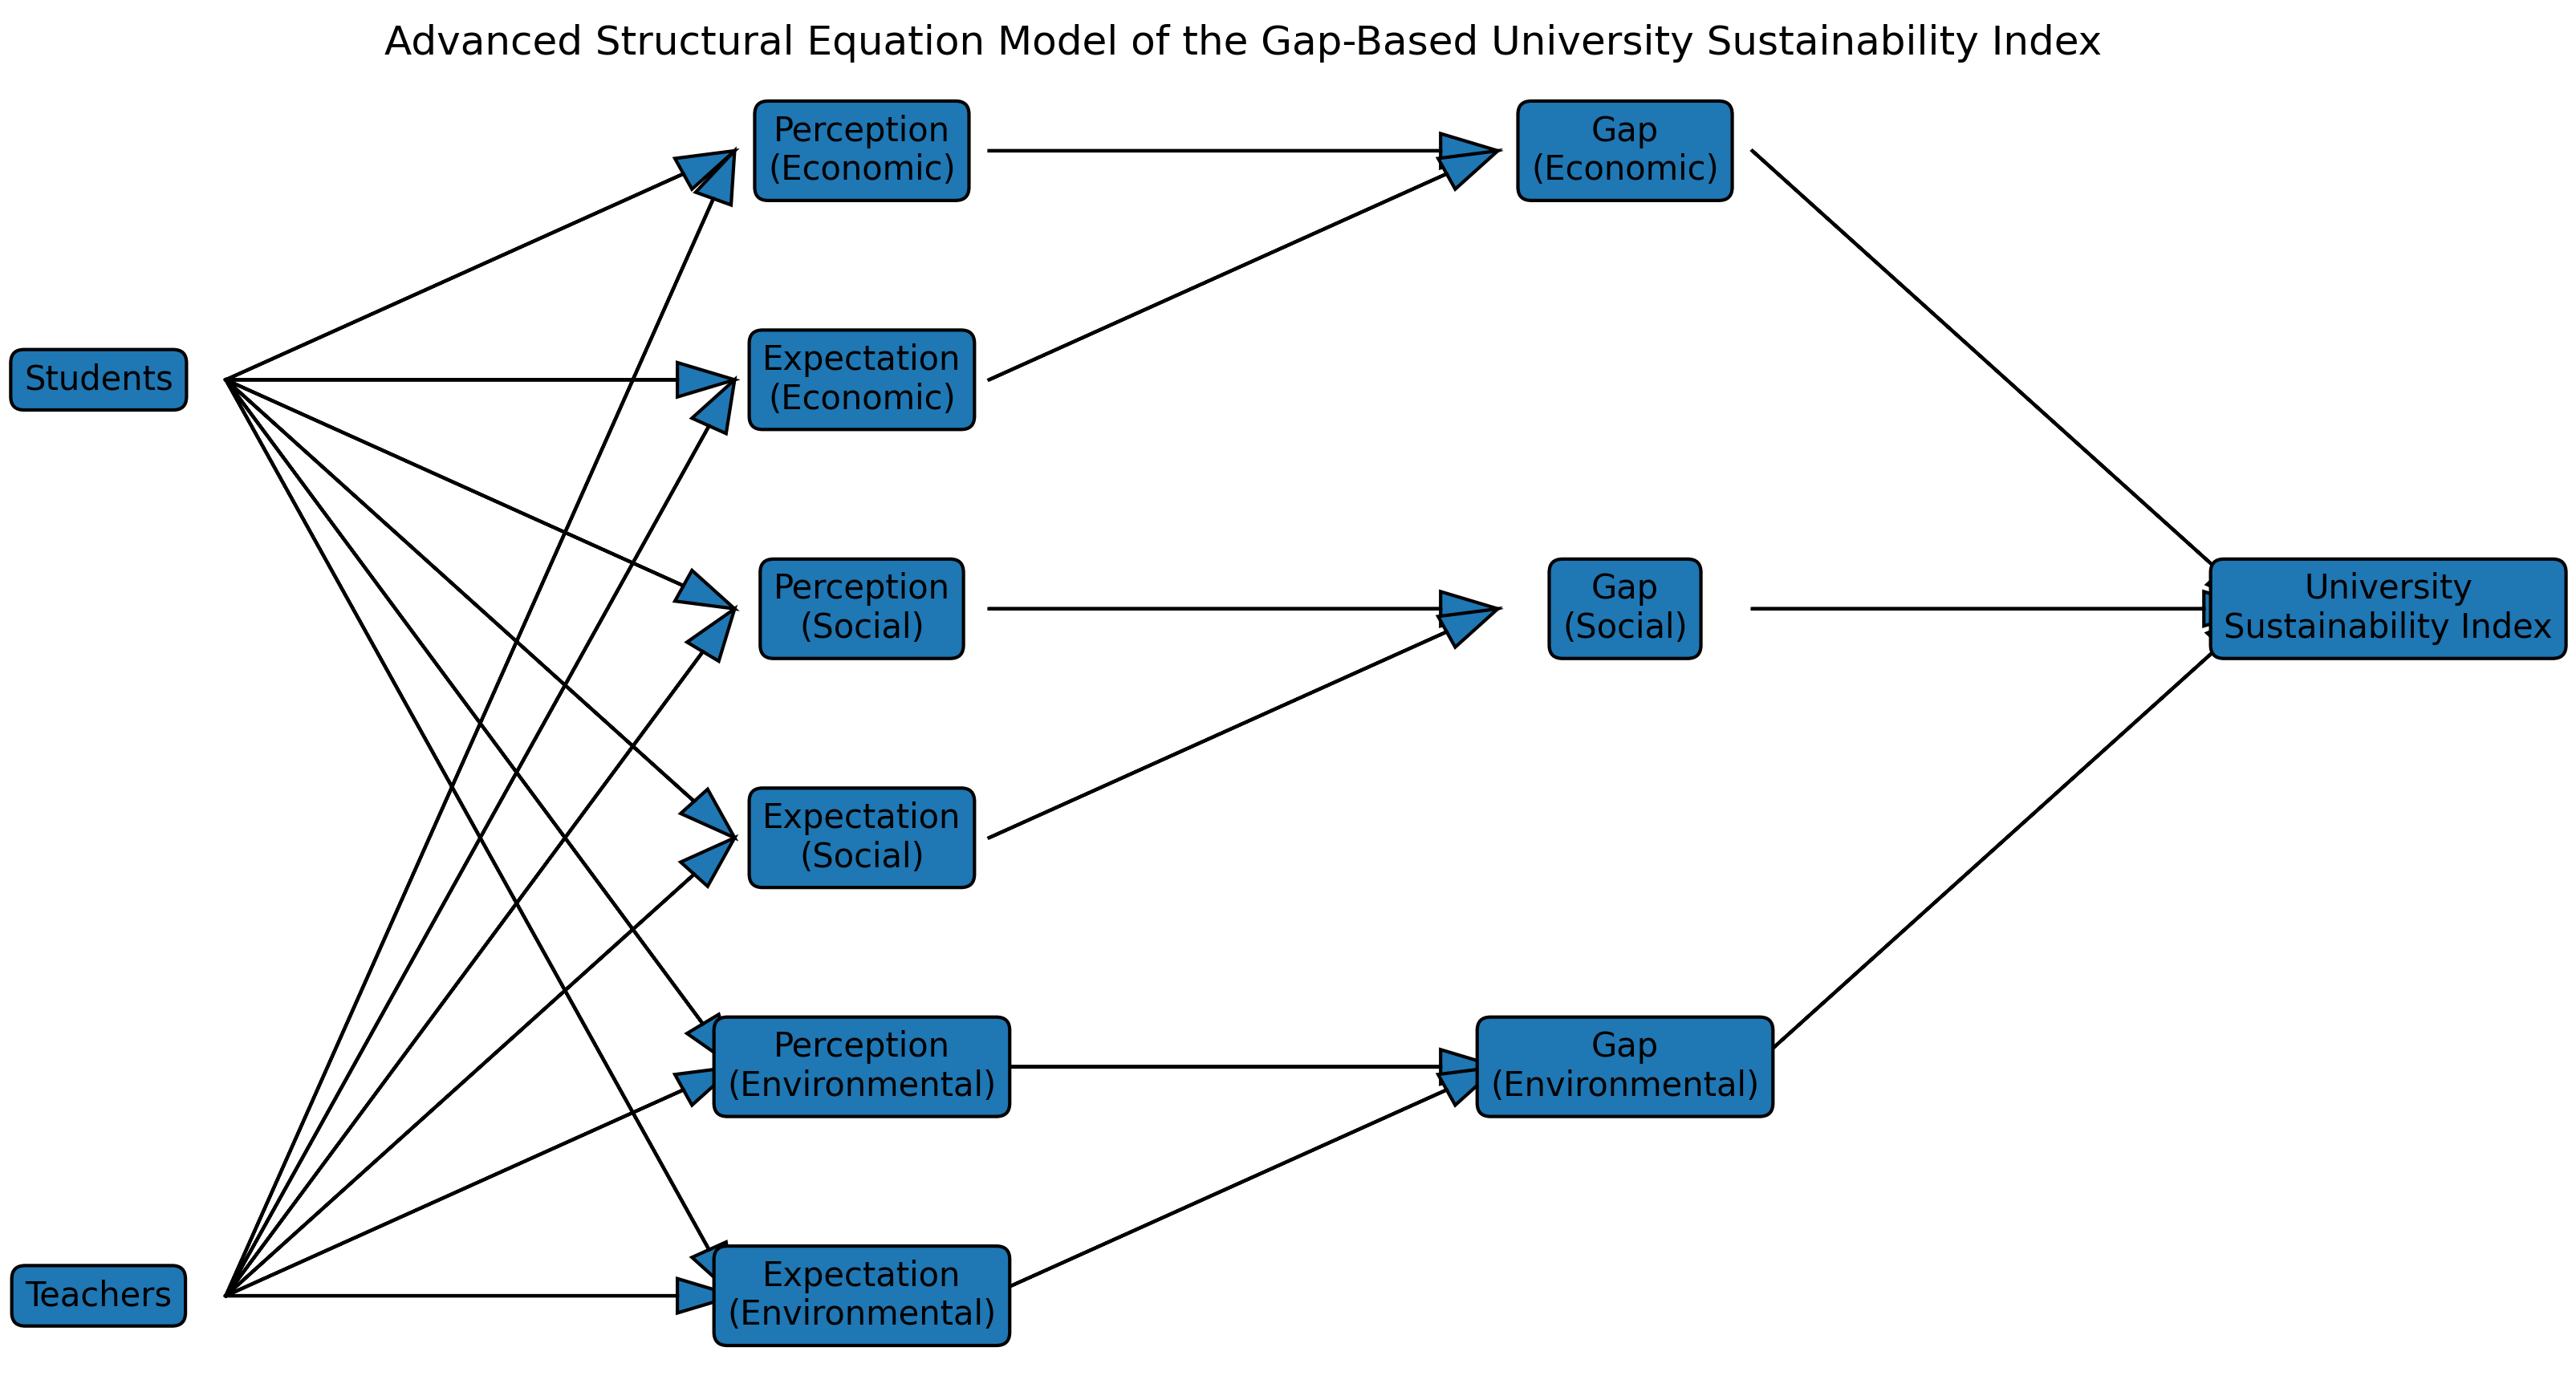
\includegraphics[width=0.8\linewidth]{Advanced_SEM_University_Sustainability_Model.png}
\caption{Structural Equation Model of the Gap-Based University Sustainability Index}
\label{fig:sem_model}
\end{figure}

The structural relationships between latent variables are formally expressed as follows:

\begin{equation}
\eta = B \eta + \Gamma \xi + \zeta
\end{equation}
In structural equation modeling, the structural relationships between latent variables are expressed in matrix form as:

\begin{equation}
\eta = B \eta + \Gamma \xi + \zeta
\end{equation}

where:

\begin{itemize}
\item $\eta$ is the vector of endogenous latent variables,
\item $\xi$ is the vector of exogenous latent variables,
\item $B$ is the matrix representing relationships between endogenous latent variables,
\item $\Gamma$ is the matrix representing relationships between exogenous and endogenous latent variables,
\item $\zeta$ is the vector of structural disturbance terms.
\end{itemize}

\subsubsection{Structural Equations for Sustainability Gaps}

The sustainability gap for each dimension is modeled as a function of perceived and expected sustainability. These relationships are defined as follows:

\begin{equation}
G_e = \gamma_{11} P_e + \gamma_{12} E_e + \zeta_1
\end{equation}

\begin{equation}
G_s = \gamma_{21} P_s + \gamma_{22} E_s + \zeta_2
\end{equation}

\begin{equation}
G_{env} = \gamma_{31} P_{env} + \gamma_{32} E_{env} + \zeta_3
\end{equation}

These equations formalize the sustainability gaps as endogenous latent constructs determined by stakeholder perception and stakeholder expectation. The gap variables capture the degree of alignment between institutional sustainability performance and stakeholder priorities.

\subsubsection{Structural Equation for the University Sustainability Index}

The University Sustainability Index is modeled as a function of the sustainability gaps across the three sustainability dimensions:

\begin{equation}
USI = \beta_1 G_e + \beta_2 G_s + \beta_3 G_{env} + \zeta_4
\end{equation}

where:

\begin{itemize}
\item $\beta_1, \beta_2, \beta_3$ represent the structural coefficients measuring the contribution of each sustainability dimension,
\item $\zeta_4$ represents the structural disturbance term associated with the sustainability index.
\end{itemize}

This equation establishes the University Sustainability Index as a higher-order latent construct integrating the sustainability gaps across economic, social, and environmental sustainability dimensions.

\subsubsection{Matrix Representation of the Structural Model}

The structural model can be expressed in matrix form as follows:

\begin{equation}
\begin{bmatrix}
G_e \\
G_s \\
G_{env} \\
USI
\end{bmatrix}
=
\begin{bmatrix}
0 & 0 & 0 & 0 \\
0 & 0 & 0 & 0 \\
0 & 0 & 0 & 0 \\
\beta_1 & \beta_2 & \beta_3 & 0
\end{bmatrix}
\begin{bmatrix}
G_e \\
G_s \\
G_{env} \\
USI
\end{bmatrix}
+
\begin{bmatrix}
\gamma_{11} & 0 & 0 & \gamma_{12} & 0 & 0 \\
0 & \gamma_{21} & 0 & 0 & \gamma_{22} & 0 \\
0 & 0 & \gamma_{31} & 0 & 0 & \gamma_{32} \\
0 & 0 & 0 & 0 & 0 & 0
\end{bmatrix}
\begin{bmatrix}
P_e \\
P_s \\
P_{env} \\
E_e \\
E_s \\
E_{env}
\end{bmatrix}
+
\begin{bmatrix}
\zeta_1 \\
\zeta_2 \\
\zeta_3 \\
\zeta_4
\end{bmatrix}
\end{equation}

\subsubsection{Interpretation of the Structural Model}

The structural model conceptualizes university sustainability as a function of stakeholder-centered alignment. Perceived sustainability and expected sustainability determine the sustainability gaps, which in turn determine the overall University Sustainability Index.

The sustainability gaps act as mediating latent variables capturing the degree of alignment between institutional sustainability performance and stakeholder expectations. Smaller gap values indicate stronger alignment and higher sustainability performance, while larger gap values indicate structural misalignment and reduced sustainability effectiveness.

This structural formulation provides a rigorous mathematical representation of sustainability as a multidimensional, stakeholder-centered construct within the structural equation modeling framework.



\subsection{Model Identification and Estimation Strategy}

The identification and estimation of the proposed structural equation model are essential to ensure the validity, reliability, and empirical applicability of the sustainability assessment framework. Model identification determines whether the model parameters can be uniquely estimated from the observed covariance matrix, while the estimation strategy defines the procedure used to obtain consistent and efficient parameter estimates.

\subsubsection{Model Identification}

A structural equation model is considered identified when each model parameter can be uniquely estimated from the covariance matrix of the observed variables \cite{Bollen1989,Kline2016}. Identification requires that the number of known elements in the observed covariance matrix exceeds the number of unknown model parameters, ensuring that a unique solution exists.

In the proposed model, identification is ensured through several structural and measurement conditions. First, each latent construct is associated with multiple observed indicators derived from stakeholder responses, which ensures measurement redundancy and construct identifiability \cite{Hair2022}. Second, scale identification is achieved by fixing one factor loading per latent variable or by constraining the variance of each latent construct, thereby defining a measurement scale for each latent variable \cite{Byrne2016}.

Furthermore, the structural model follows a recursive formulation, where sustainability gaps are determined by perceived and expected sustainability, and the University Sustainability Index is determined by the sustainability gap constructs. This recursive structure eliminates feedback loops and ensures model identification \cite{Kline2016}. Since the number of observed variances and covariances exceeds the number of free parameters, the proposed model is over-identified, allowing empirical estimation and statistical testing.

\subsubsection{Estimation Method}

The estimation of the structural equation model parameters can be performed using covariance-based structural equation modeling (CB-SEM) or partial least squares structural equation modeling (PLS-SEM), depending on the research objectives and data characteristics.

In covariance-based SEM, Maximum Likelihood (ML) estimation is commonly used to estimate model parameters by minimizing the discrepancy between the observed covariance matrix and the model-implied covariance matrix \cite{Kline2016,Byrne2016}. Maximum Likelihood estimation provides efficient and asymptotically unbiased parameter estimates under standard statistical assumptions.

Alternatively, Partial Least Squares Structural Equation Modeling (PLS-SEM) can be used when the research objective emphasizes prediction and when distributional assumptions are less restrictive \cite{Hair2022}. PLS-SEM is particularly suitable for complex models involving multiple latent constructs and stakeholder-based sustainability assessments.

\subsubsection{Parameter Estimation and Model Evaluation}

The estimation process determines the parameters defining both the measurement model and the structural model. These parameters include:

\begin{itemize}
\item Factor loadings ($\Lambda_x$, $\Lambda_y$), which define the relationships between observed indicators and latent variables;
\item Structural coefficients ($B$, $\Gamma$), which define the relationships between latent variables;
\item Measurement error variances ($\delta$, $\epsilon$);
\item Structural disturbance variances ($\zeta$).
\end{itemize}

Measurement reliability and validity are evaluated using established SEM criteria, including factor loadings, composite reliability, and convergent validity \cite{Fornell1981,Hair2022}. Structural validity is assessed through the magnitude and statistical significance of structural coefficients.

Model fit can be evaluated using standard fit indices such as the Comparative Fit Index (CFI), Tucker–Lewis Index (TLI), Root Mean Square Error of Approximation (RMSEA), and Standardized Root Mean Square Residual (SRMR), which provide quantitative measures of model adequacy \cite{Kline2016,Byrne2016}.

This identification and estimation strategy ensures that the proposed gap-based structural equation model provides a statistically valid and empirically estimable framework for assessing university sustainability from a stakeholder-centered perspective.

\subsection{Theoretical Contribution of the Gap-Based Sustainability Model}

The proposed gap-based structural equation model introduces a novel conceptual and methodological framework for assessing university sustainability from a stakeholder-centered perspective. Unlike traditional sustainability assessment approaches that primarily rely on objective operational indicators, the proposed model integrates perceptual, motivational, and alignment-based dimensions into a unified structural representation.

First, the model conceptualizes sustainability as a multidimensional latent construct structured around economic, social, and environmental dimensions, reflecting the holistic nature of institutional sustainability. This formulation extends existing sustainability assessment frameworks by incorporating stakeholder-centered latent constructs inferred from perceptual and expectation-based evaluations.

Second, the introduction of the Expectation--Perception Gap as a mediating latent construct represents a key theoretical contribution. The gap construct captures the degree of alignment between institutional sustainability initiatives and stakeholder expectations, thereby providing a behavioral and relational interpretation of sustainability performance. This perspective shifts the evaluation of sustainability from a purely operational paradigm toward an alignment-based paradigm, where sustainability effectiveness depends not only on institutional actions but also on their perceived adequacy relative to stakeholder priorities.

Third, the proposed model establishes the University Sustainability Index as a higher-order latent construct integrating the sustainability gaps across multiple sustainability dimensions. This index provides a mathematically grounded and structurally consistent measure of sustainability that reflects both institutional performance and stakeholder-centered alignment. By integrating perceptual, expectation-based, and structural dimensions, the index offers a more comprehensive representation of sustainability than traditional indicator-based assessment methods.

Fourth, the structural equation modeling formulation provides a rigorous quantitative framework that enables empirical estimation, statistical validation, and predictive analysis of sustainability performance. The integration of measurement and structural components ensures construct validity, reliability, and theoretical consistency.

Overall, the proposed model advances the theoretical understanding of university sustainability by introducing a gap-based structural formulation that explicitly integrates stakeholder perception, stakeholder expectation, and institutional sustainability performance into a unified latent variable framework. This approach establishes a new foundation for stakeholder-centered sustainability assessment and provides a scalable and empirically testable framework for sustainability evaluation in higher education institutions.

\bibliographystyle{apacite}
\bibliography{references}

\end{document}